\begin{comment}

Source: https://redmine.upd89.org/redmine/projects/upd89/wiki/API

\end{comment}

\section{API}

Die beiden Komponenten \gls{agent} und \gls{controlcenter} kommunizieren über eine API.

\subsection{Control Center}

\begin{table}[]
\centering
\caption{API-Endpunkte auf Seite Control Center}
\label{api:endpoints}
\begin{tabular}{ll}
\hline
\textbf{Aufruf}                     & \textbf{Details}                                  \\ \hline
/register                           & A registriert sich beim CC                        \\
/system/:urn/notify-hash            & A teilt seine anstehenden Updates mit CC via Hash \\
/system/:urn/notify                 & siehe oben, aber mit vollständigen Informationen  \\
/system/:urn/refresh-installed-hash & A meldet CC seine installierten Pakete als Hashes \\
/system/:urn/refresh-installed      & siehe oben, aber mit vollständigen Informationen  \\
/task/:id/notify                    & A meldet Status zu spez. Task                     \\ \hline
\end{tabular}
\end{table}

\subsection{Status-Codes}

\begin{table}[]
\centering
\caption{Status-Codes}
\label{api:codes}
\begin{tabular}{ll}
\hline
\textbf{Status} & \textbf{Bedeutung}                                                          \\ \hline
OK              & Alles war in Ordnung                                                        \\
ERROR           & Fehler im Ablauf                                                            \\
infoIncomplete  & Mind. 1 der Hashes ist unbekannt                                            \\
countMismatch   & System hat eine andere Anzahl installierte Pakete/Updates als gemeldet      \\
pkgUnknown      & Mindestens eines der gemeldeten Pakete oder Base-Versions ist nicht bekannt \\ \hline
\end{tabular}
\end{table}


\begin{figure}
  \centering
    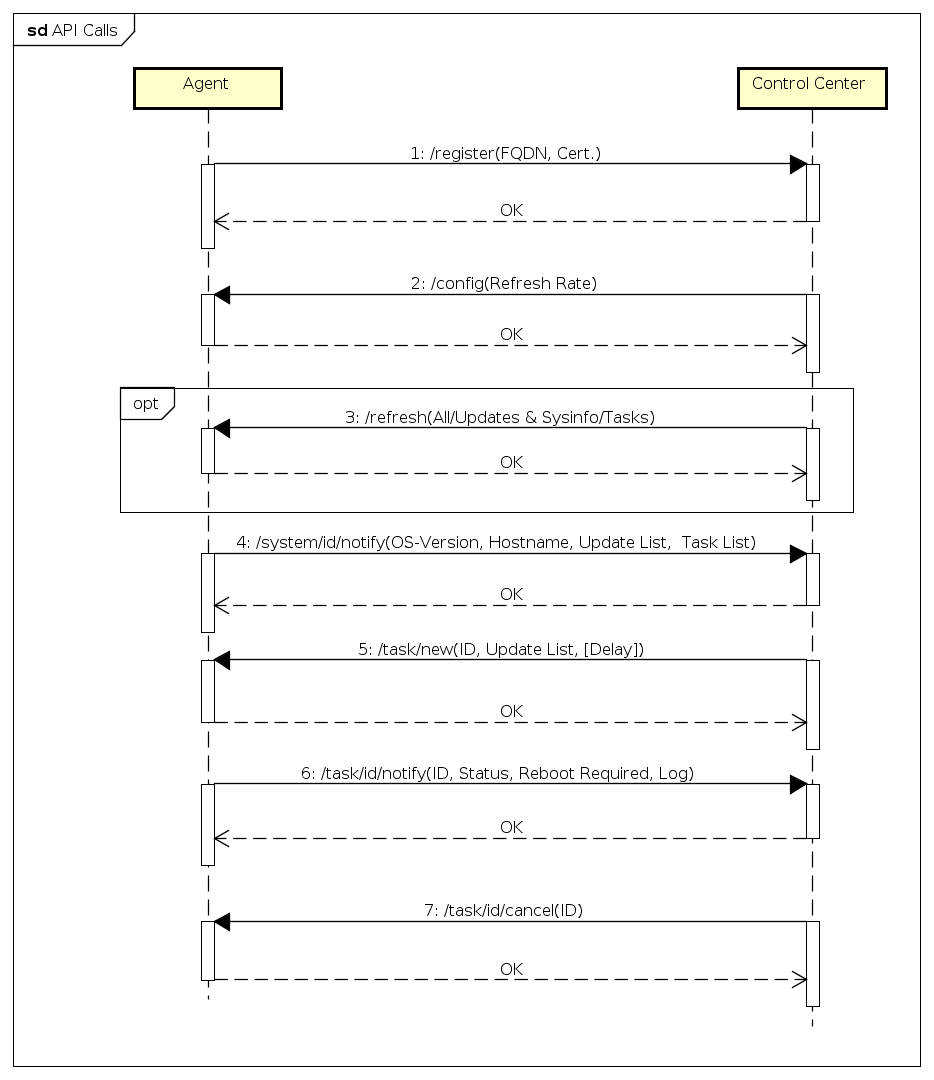
\includegraphics[width=\textwidth]{fig/API_Calls}
  \caption{Sequenzdiagramm bezüglich API-Aufrufe}
  \label{fig:api_sequence_diagram}
\end{figure}

\subsubsection{/register}